\section{Introduction}
\label{sec:unsupervised_intro}
The application of modern deep learning algorithms has demonstrated significant improvements in digital pathology tasks such as nuclei detection and disease classification~\citep{litjens2017survey}, as previously discussed in Section \ref{subsec:active_for_medical_image_analysis}. The ability to jointly learn deep representations and discriminative classifiers or regressors through end-to-end training allows for feature representations that are specifically tailored to a given task. However, this approach necessitates a significant amount of annotated data for adequate generalisation, which poses a major challenge for digital pathology~\citep{madabhushi2016image} and other medical image analysis domains. In an effort to address this challenge, we previously explored the use of active learning (Chapter \ref{ch:active_learning}), however, the limitations of this approach were highlighted in Section \ref{sec:active_conclusion} and subsequently led to a focus on unsupervised representation learning as a means to extract information from unannotated images. Unsupervised representation learning can be utilised to improve generalisation, decrease data dimensionality, improve computational performance, and initialise deep supervised learning models when access to annotated data is limited~\citep{bengio2013representation}.

\begin{figure}
	\begin{minipage}[b]{.4\linewidth}
		\centering
		\centerline{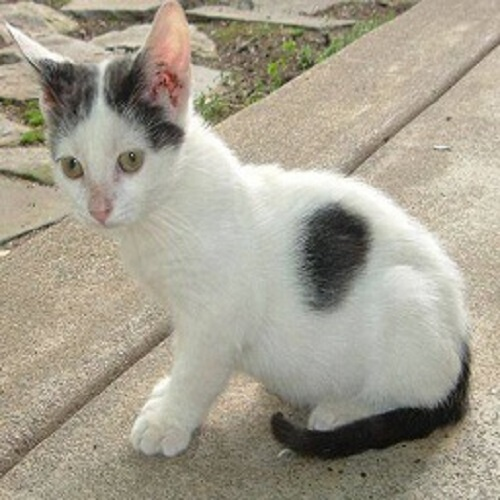
\includegraphics[width=\textwidth]{images/cat.jpg}}
		\centerline{(a)}\medskip
	\end{minipage}
	\hfill
	\begin{minipage}[b]{0.4\linewidth}
		\centering
		\centerline{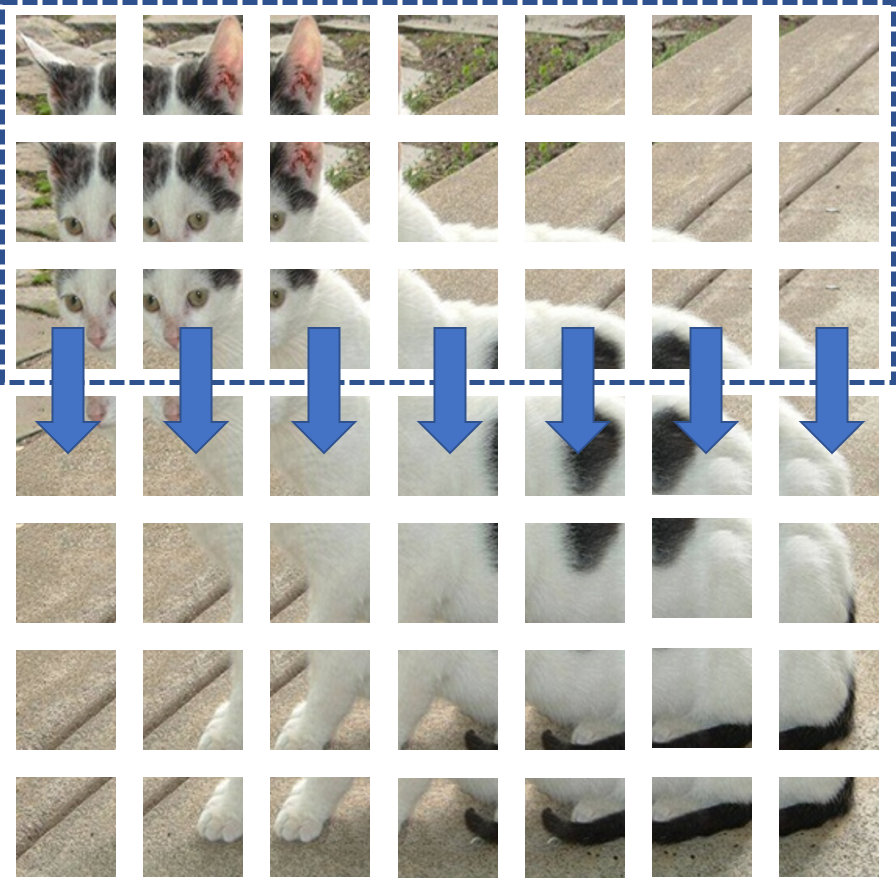
\includegraphics[width=\textwidth]{images/cat_grid_v2.png}}
		\centerline{(b)}\medskip
	\end{minipage}
	\\
	\begin{minipage}[b]{.4\linewidth}
		\centering
		\centerline{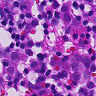
\includegraphics[width=\textwidth]{images/histo.png}}
		\centerline{(c)}\medskip
	\end{minipage}
	\hfill
	\begin{minipage}[b]{.4\linewidth}
		\centering
		\centerline{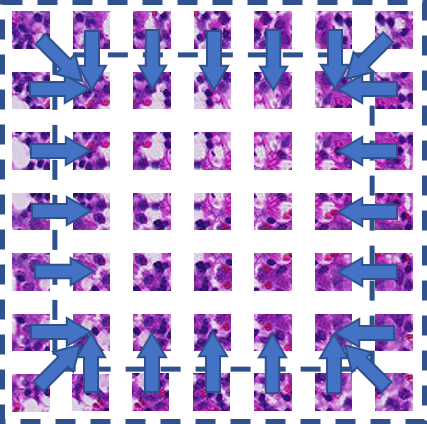
\includegraphics[width=\textwidth]{images/histo_grid.png}}
		\centerline{(d)}\medskip
	\end{minipage}
	\caption{(a) An example image from the ImageNet dataset~\citep{deng2009imagenet}. (b) Extracted overlapping patches with those used to produce context and autoregressor direction highlighted. (c) An example image from the Patch Camelyon dataset~\citep{veeling2018rotation}. (d) Extracted overlapping patches with those used to produce context and autoregressor direction highlighted.}
	\label{fig:example_cpc_patches}
\end{figure}

One approach to reducing the need for large, annotated datasets is through the use of unsupervised representation learning and transfer learning. This is accomplished by using the weights of a deep encoder, trained on a large pool of unannotated data, to initialise another model~\citep{weiss2016survey}. Contrastive predictive coding (CPC) is a state-of-the-art method for unsupervised representation learning~\citep{oord2018representation}. It involves training an autoregressive model to predict future data representations in a sequence, using a loss function with noise-contrastive estimation and importance sampling components, to preserve the density ratio between each sample and its representation. Although originally developed for sequential data, CPC has been adapted for images by splitting each image into overlapping patches and using an encoder to produce a matrix of feature representations. A mask is then applied to the matrix so that an autoregressive model can only see a subset of the feature representations in order to predict the representations of the masked patches from the context available to it. This framework has been applied successfully to object detection and Imagenet classification tasks with modifications to model capacity, layer normalisation, prediction directions, and patch-based augmentations~\citep{henaff2019data}. However, in previous implementations, the autoregressive model’s predictions were made in multiple directions individually, which can be inefficient when dealing with images, such as in digital pathology, where the orientation of the image is arbitrary and does not carry useful information. Figure~\ref{fig:example_cpc_patches}(b) illustrates an example of this framework applied to an image.

\begin{figure}[b]
	\centering
	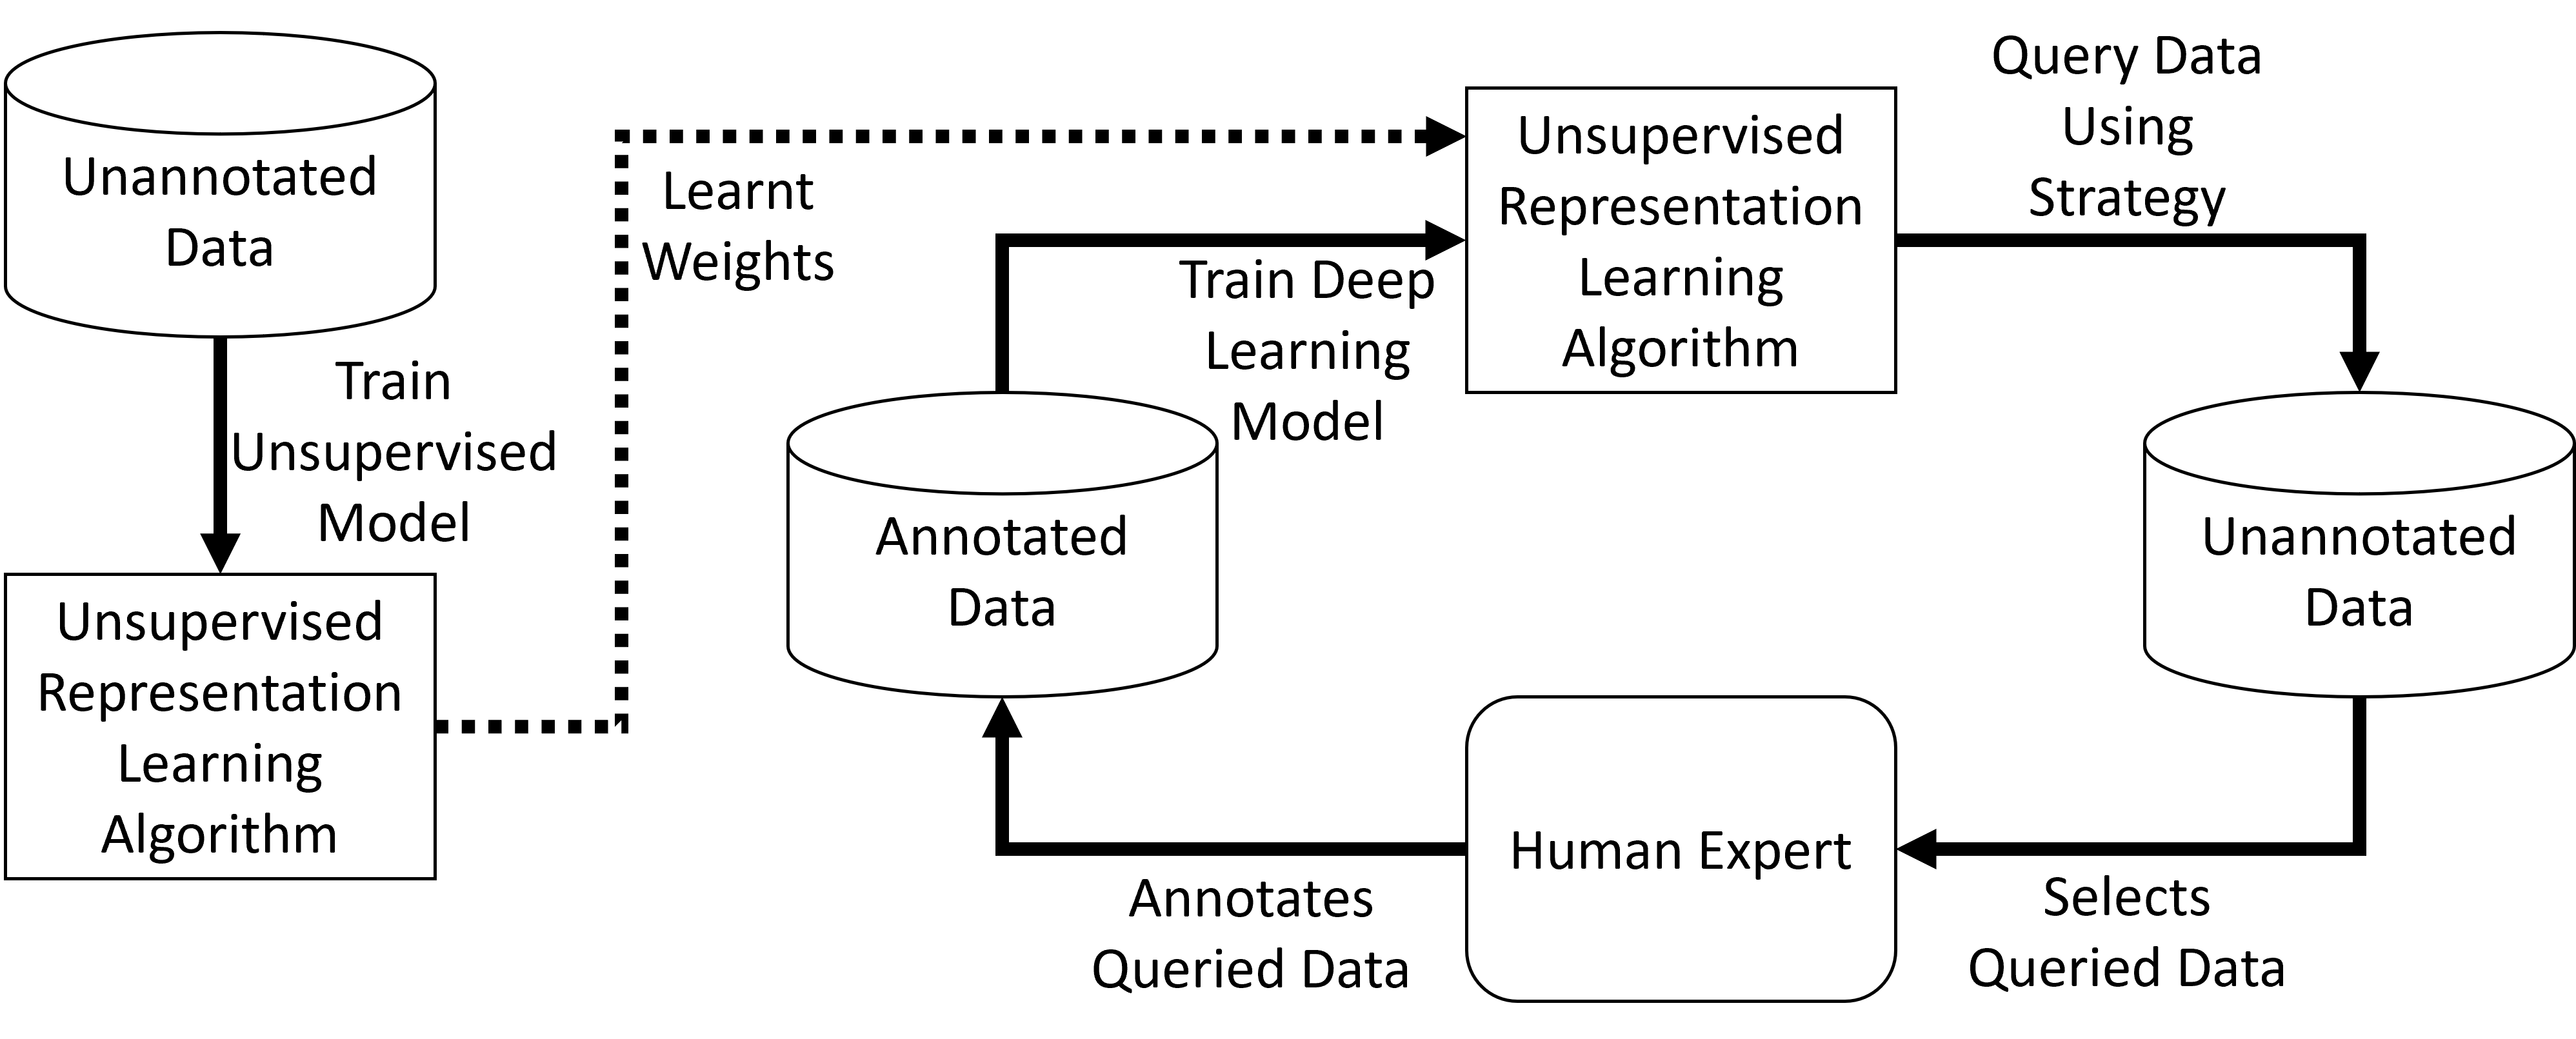
\includegraphics[width=\textwidth]{images/active_unsupervised_learning.png}
	\caption{Proposed active learning framework with learnt representations from unsupervised representation learning on unannotated data.}
	\label{fig:active_unsupervised_learning_framework}
\end{figure}

The current study builds upon the idea that unsupervised representation learning can be utilised to learn deep representations, which can then be used in conjunction with transfer learning to train a discriminative classifier with limited annotated data (as depicted in Figure~\ref{fig:active_unsupervised_learning_framework}). By implementing this approach, the need for complex deep learning-specific active learning query strategies is mitigated and instead allows for a focus on uncertainty-based querying. In order to realise this approach, a state-of-the-art unsupervised representation learning algorithm for digital pathology images was required. To this end, a multi-directional CPC extension was proposed, which includes an alternative mask for building latent context and a new extension to the autoregressive model PixelCNN~\citep{oord2016pixel} for multi-directional predictions (as depicted in Figure~\ref{fig:example_cpc_patches}(d)). The effectiveness of this modification was demonstrated using the PatchCamelyon dataset~\citep{veeling2018rotation}, derived from the Camelyon16 dataset~\citep{litjens20181399}, where it was shown that classification can be performed with less annotated data when utilising representations learned in this way. 

This work was presented at the IEEE International Symposium on Biomedical Imaging 2021 and published as part of its proceedings \citep{carse2021unsupervised}.



\section{Unsupervised Representation Learning for Computer Vision}
\label{subsec:unsupervised_representation}
In the field of deep learning, methods have shown exceptional performance in tasks involving abundant labelled data. However, their performance is known to suffer in scenarios where the supervision is limited. One solution to this issue is to utilise unsupervised learning techniques to learn highly structured data representations, which can lead to more data-efficient models~\citep{lake2015human}.

Deep learning models typically consist of layers that are used for specific tasks, such as classification or regression, and others that are used to encode the data into feature representations, known as encoders. Unsupervised representation learning in deep learning focuses on learning the parameters of the encoder. Once trained, the encoder can be used for transfer learning and applied to tasks such as classification, object detection, or segmentation~\citep{weiss2016survey}.

In the context of computer vision, there are two main approaches to deep representation learning: generative methods and self-supervised learning~\citep{bengio2013representation}. Generative methods aim to learn representative feature encodings by attempting to reconstruct images. On the other hand, self-supervised learning involves training models in a supervised manner using auto-generated labels for classification or regression tasks.

\subsection{Generative Methods}
\label{subsec:generative_methods}
Generative models, a class of machine learning algorithms, have been widely adopted for representation learning, as they can learn to generate new data samples that are similar to the training data. In particular, in the context of medical image analysis, generative models have been used for image-to-image translation tasks, such as converting images from one modality to another~\citep{kaji2019overview}. The increasing popularity of generative models in medical image analysis can be attributed to their ability to learn useful representations from large amounts of unlabelled data, which can subsequently be utilised to improve performance on tasks such as segmentation and classification~\citep{yi2019generative}.

\subsubsection{Autoencoders}
\label{subsubsec:autoencoders}
Autoencoders are a class of generative models that employ an encoder to reduce the dimensionality of the input data and a decoder to reconstruct the original data from the reduced representation~\citep{kramer1991nonlinear}. Transfer learning can be achieved by utilising the parameters learned by the encoder and training a new classifier with the encoded representations. One of the most widely used types of autoencoders is the undercomplete autoencoder, which is trained to minimise the reconstruction error by learning a compressed feature representation~\citep{goodfellow2016deep}. Other variations of autoencoders include sparse autoencoders, which are designed to learn sparse representations that have been shown to improve performance when used for transfer learning~\citep{makhzani2013k}. Denoising autoencoders, on the other hand, are trained by corrupting the input data with noise and the goal of the network is to reconstruct the original data without the added noise. This denoising training process forces the encoder and decoder to implicitly learn the underlying structure of the data, which can be beneficial for transfer learning~\citep{bengio2013generalized}.

The final category of autoencoder is the regularised autoencoder, which modifies the traditional autoencoder architecture in order to enhance the model's ability to learn more informative representations and capture relevant information. One of the most widely employed forms of regularised autoencoder is the variational autoencoder, as proposed by \cite{kingma2013auto}. This variant of autoencoder ensures that the latent space possesses desirable properties that enable a generative process by encoding an input image as a distribution over the latent space, as opposed to encoding it into a single point in the latent space. A variational autoencoder is trained by sampling from the encoded latent distribution and decoding it into an output image. The loss function for this model is based on the reconstruction error of the output image and the Kulback-Leibler divergence~\citep{kullback1951information} as the regularisation term.

Most recent work with autoencoders in medical image analysis has been using variational autoencoders as they have shown a high level or performance and have been used for multiple tasks~\citep{wei2020recent}. \cite{akrami2020brain} used a combination of variational autoencoders and transfer learning to build unsupervised lesion detection models for MRI brain scans images and showed their robustness when working with training and testing datasets with different parameters~\citep{thiagarajan2020improving}. 

\subsubsection{Generative Adversarial Networks}
\label{subsubsec:generative_adversarial_networks}
Generative adversarial networks~\citep{goodfellow2014advances} are a class of deep learning models that are designed to generate new samples of data that resemble existing samples from a given dataset. They consist of two main components: a generator network, which produces new samples, and a discriminator network, which attempts to distinguish the generated samples from the real samples. The two networks are trained in an adversarial manner, with the generator attempting to produce samples that the discriminator cannot distinguish from real samples, and the discriminator attempting to correctly identify the generated samples. However, generative adversarial networks are known to be difficult to train, one common problem when training generative adversarial networks is mode collapse, where the generator produces a limited set of outputs that fail to capture the full diversity of the real data distribution. Several techniques, such as Wasserstein generative adversarial networks~\citep{arjovsky2017wasserstein} and gradient penalty~\citep{gulrajani2017improved} have been proposed to stabilise the training process.

In the context of representation learning, generative adversarial networks can be used to learn a compact, low-dimensional representation of the data that captures the underlying structure of the dataset. This can be achieved by training the generator to produce samples that are similar to the real samples, but in a lower-dimensional space. The generator can then be used as a feature extractor, mapping the real samples to their corresponding low-dimensional representations. Additionally, the discriminator can be used as a classifier, allowing the learned representations to be used for downstream tasks such as classification~\citep{srivastav2021improved} or clustering~\citep{mukherjee2019clustergan}.

A variant of generative adversarial networks is BigBiGAN~\citep{donahue2019large}, which is designed to generate high-quality images from a compact, low-dimensional representation of the data. It is based on the idea of BiGAN~\citep{donahue2016adversarial} and the primary difference between BigBiGAN and the original BiGAN is the scale of the model. BigBiGAN is trained on a large dataset such as ImageNet, which contains millions of images, whereas BiGAN is trained on smaller datasets. The increased size of the dataset allows BigBiGAN to learn a more powerful and expressive representation of the data. BigBiGAN consists of three main components: an encoder network, a generator network, and a discriminator network. The encoder network maps the input data to a low-dimensional representation, which is then used as input to the generator network to produce a reconstructed sample.

\subsection{Self-supervised Methods}
\label{subsec:self_supervised_methods}
Self-supervised learning for representation learning is a subset of machine learning that aims to learn meaningful representations of data without the need for explicit labels. A prevalent method for self-supervised representation learning in medical imaging is to employ a pretext task, a task that is simple to solve through the utilisation of the features learned by the model, but also serves as a means to learn relevant features for the ultimate task of interest. The utilisation of self-supervised pre-training techniques is rapidly gaining popularity in medical image analysis, as it enables the learning of useful features from vast amounts of unlabelled data, which can then be applied to enhance performance in tasks such as segmentation and classification~\citep{shurrab2022self}.

\subsubsection{RotNet}
\label{subsubsec:RotNet}
RotNet, as proposed by \cite{gidaris2018unsupervised}, is a novel unsupervised representation learning technique that utilises rotation as a self-supervised task for learning useful representations of images. The fundamental concept behind RotNet is that by training a neural network to predict the rotation of an image, it can learn useful features that are rotation-invariant and can be utilised in other tasks such as image classification. The RotNet model comprises of a convolutional neural network that takes an image as input and predicts the angle of rotation. The output of the last convolutional layer, prior to the fully connected layers, is used as the representation of the image. This technique enables the model to train on a large dataset of unannotated images, which can then be utilised for other tasks such as image classification as demonstrated by \cite{zhou2021preservational}.

\subsubsection{Deep Clustering}
\label{subsubsec:deep_clustering}
DeepCluster, as proposed by \cite{caron2018deep}, is a technique for unsupervised representation learning that combines the utilisation of clustering algorithms as a form of self-supervision to train deep neural networks. The method initiates by initialising the weights of a deep neural network randomly and subsequently utilising the network to extract features from a dataset of unlabelled images. These features are then employed to cluster the images into different groups using a clustering algorithm, such as k-means. Upon completion of the clustering process, the labels generated by the clustering algorithm are used as pseudo-labels for the images. The neural network is then fine-tuned using these pseudo-labels to enhance the representations of the images. This process is repeated multiple times, with the neural network being fine-tuned using the updated pseudo-labels generated by the clustering algorithm.

\subsubsection{Non-Parametric Instance-Level Discrimination}
\label{subsubsec:non-parametric_instance-level_discrimination}
Non-parametric instance-level discrimination is a method for unsupervised representation learning that focuses on learning a set of discriminative features that can be used to differentiate between individual instances in a dataset. This approach is non-parametric, meaning that it does not rely on any assumptions about the underlying distribution of the data or the form of the learned features. \cite{wu2018unsupervised} purposed a modification to apply this to deep learning. The authors noted that simply extended the softmax output to the size of the dataset is not feasible and instead found a way around this by approximating the softmax distribution using noise-contrastive estimation~\citep{gutmann2010noise} and using proximal regularisation method~\citep{parikh2014proximal}.

\subsubsection{Local Aggregation}
\label{subsubsec:local_aggregation}
In their work, \cite{zhuang2019local} proposed a method for unsupervised representation learning using local non-parametric aggregation in the latent feature space. The proposed method is based on training an encoder to produce latent features, and encouraging similar data instances to move together and dissimilar instances to separate in the latent feature space. To achieve this, the method employs a clustering technique. Specifically, multiple passes of k-means clustering are performed for each latent encoding to determine its close neighbours and background neighbours. The loss function used to train the model is based on the negative log-likelihood of an encoding being recognised as a close neighbour, given that it is recognised as a background neighbour. The effectiveness of the proposed method is demonstrated through experiments on the Imagenet dataset~\citep{deng2009imagenet}. The results show that the model trained with this method exhibits substantial ability to recognise high-level visual context without the need for any dataset annotations. This highlights the potential of the proposed method for unsupervised representation learning in computer vision tasks.

\subsubsection{Momentum Contrast}
\label{subsubsec:momentum_contrast}
In their work, \cite{he2020momentum} proposed a method for unsupervised representation learning called momentum contrast. The method uses a dynamic dictionary of keys to train an encoder. Specifically, the encoder is trained using a contrastive loss, which compares the representation of a query image to the key representations from the dynamic dictionary, which is made up of a queue of data samples. The authors claim that the use of a large and dynamic dictionary allows for an effective sampling of high-dimensional visual space, which results in competitive performance. This is supported by the experimental results presented in the work, which show that the learned feature representations can be used to pre-train encoders for a variety of tasks such as classification, detection, and segmentation. This highlights the potential of the Momentum Contrast method for unsupervised representation learning in computer vision tasks.

\subsubsection{Pretext-Invariant Representations}
\label{subsubsec:pretext_invariant_representations}
In a recent study, \cite{misra2020self} highlighted a limitation of using pretext tasks for self-supervised representation learning, specifically that it can result in overfitting and poor generalisation to other tasks. To address this issue, the authors proposed a novel approach called pretext-invariant representation learning. This method involves applying a transformation, such as a rotation, to an input image, and then encoding both the original and transformed images using a shared encoder. The final embeddings are generated using separate prediction heads. To further improve the robustness of the learned representations, the authors employed a noise contrastive estimator~\citep{gutmann2010noise} as the loss function, which aims to reduce the similarity between the original and transformed images, while maximising the similarity between the transformed image and randomly sampled negative images. The encoder used in the study was a ResNet~\citep{he2016deep}, and the authors demonstrated the effectiveness of the proposed approach by achieving state-of-the-art results using a jigsaw pretext task~\citep{noroozi2016unsupervised} in their method.

\subsubsection{Deep InfoMax}
\label{subsubsec:DIM}
Deep infomax, first proposed in~\citep{hjelm2018learning}, is a self-supervised deep learning approach for learning compact and informative representations of data through the optimisation of mutual information between the data and the learned representations. Mutual information is a measure of the dependence between two random variables and quantifies the amount of information that one variable contains about the other. In the case of deep infomax, the data is considered as one random variable and the learned representation as the other. The mutual information between the data and the learned representation is estimated using a variational lower bound.

An extension of this approach, Augmented Multiscale Deep InfoMax (AMDIM)~\citep{bachman2019learning}, aims to learn hierarchical representations of data by utilising a multiscale architecture. This architecture is composed of multiple sub-networks, each responsible for learning representations at a different scale. The decoder network also comprises of multiple sub-networks, each responsible for reconstructing the data from the representations at a corresponding scale. Like deep infomax, the mutual information between the data and the learned representations is estimated using a variational lower bound. The key difference between deep infomax and AMDIM is that the latter utilises multiple scales to learn hierarchical representations, while the former only uses one scale. The authors of the paper have demonstrated state-of-the-art results using transfer learning to train classifiers.

\subsection{Unsupervised Representation Learning for \\Medical Image Analysis}
\label{subsec:unsupervise_representation_for_medical}
In the field of digital pathology, transfer learning is a widely used technique for various tasks~\citep{srinidhi2020deep}, as it has been shown to accelerate the convergence of deep learning models~\citep{bayramoglu2016transfer}. Studies have also demonstrated the effectiveness of utilising representation learning to initialise a CNN in situations where the learning task may be challenging due to a lack of annotated data~\citep{hou2016automatic}. This approach can also be extended to active learning, where limited annotations make it difficult to learn features effectively~\citep{carse2019active}.

Instead of relying on features trained on general computer vision data, some researchers have explored the use of more general histology features for cell-level tasks~\citep{hu2018unsupervised}. One method for achieving this is by training a unified generative adversarial network with a modified loss function for cell-level representation learning. Another approach is to use multi-scale convolutional sparse coding, which aims to jointly learn features at different scales with enforced scale-specificity~\citep{chang2017unsupervised}.




\section{Multi-Directional Contrastive Predictive Coding}
\label{sec:unsupervised_multi_directional_cpc}
\subsection{Contrastive Predictive Coding}
\label{subsec:unsupervised_cpc}
Contrastive Predictive Coding (CPC) is a method for learning feature representations in an unsupervised manner from sequential data. The CPC method is based on the idea of predicting future representations from past representations, thereby allowing the model to learn "slow" features that effectively represent the underlying input data distribution \citep{henaff2019data,oord2018representation}. A CPC model consists of two main components: an encoder $g_{en}$ that encodes each element $x_t$ of the input sequence $x$ into a latent representation $z_t = g_{en}(x_t)$, and an autoregressive model $g_{ar}$ that summarizes part of the latent representation sequence $z_{\le t}$ into a latent context representation $c_t = g_{ar}(z_{\le t})$. Instead of using the autoregressive model to predict future samples, a density ratio is modeled, which preserves the mutual information between $x_{t+k}$ and $c_t$ (as described in Equation\ref{eq:density_ratio}).

\begin{equation}
	f_k(x_{t+k}, c_t) \propto \frac{p(x_{t+k}|c_t)}{p(x_{t+k})}
	\label{eq:density_ratio}
\end{equation}

Direct evaluation of $p(x)$ or $p(x|c)$ is not possible, but since the distribution can be sampled, Noise-contrastive estimation \citep{gutmann2010noise} can be employed by comparing a target value to random negative samples. The loss function used to jointly optimize the encoder and autoregressive models is called InfoNCE (as described in Equation\ref{eq:InfoNCE}), it is based on Noise-contrastive estimation. The loss function uses a set $X={x_i,…,x_N}$ of $N$ random samples, containing one positive sample from $p(x_{t+k}|c_t)$ and $N-1$ negative samples from $p(x_{t+k})$. By optimizing this loss function, the result will be $f_k(x_{t+k}, c_t)$, which estimates the density ratio from Equation~\ref{eq:density_ratio}.

\begin{equation}
	L=-\underset{x}{\mathbb{E}}\left[\log\frac{f_k(x_{t+k},c_t)}{\sum_{x_j\in X}f_k(x_j,c_t))}\right]
	\label{eq:InfoNCE}
\end{equation} 

\subsection{Contrastive Predictive Coding for Computer Vision}
\label{subsec:unsupervised_cpc_for_vision}
CPC is a method originally proposed for sequential data, and its application to computer vision involves first dividing an input image into overlapping patches. Each patch is then encoded, and an autoregressive model is employed to generate a context vector from the patch representations at the top of the image (as depicted in Figure~\ref{fig:example_cpc_patches}(b), where the top 3 rows of patches were utilised~\citep{oord2018representation}). This approach treats each column of the image as a sequence, with the context vector from the top of the image used to model the density ratio with patch representations below. This technique has been demonstrated to achieve data-efficient results on high-level computer vision datasets, such as Imagenet~\citep{deng2009imagenet}.

\subsection{Multi-Directional Contrastive Predictive Coding}
\label{subsec:unsupervised_mdcpc}
The approach of treating columns of the representation matrix as individual sequences (as described in Section~\ref{subsec:unsupervised_cpc_for_vision}), can negatively impact performance when working with images where image orientation is irrelevant, such as histology patches or dermoscopic skin lesion images. While the orientation of certain histology whole slide images can be biologically meaningful, the orientation of image patches, such as those shown in Figure~\ref{fig:example_cpc_patches}(c) (sentinel lymph node) orientation, is not important. In such cases, the autoregressive model can struggle to predict patch representation from the provided context as the vertical image axis is arbitrary, unlike Imagenet where it correlates with the direction of gravity acting upon the image content.

\begin{figure}
	\centering
	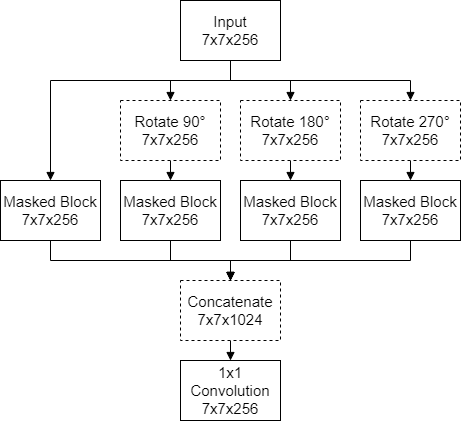
\includegraphics[width=0.9\textwidth]{mcb.png}
	\caption{Architecture of a Multi-Directional Masked Block}
	\label{fig:multi-directional_masked_block}
\end{figure}

To address this limitation, this work proposes two modifications inspired by image in-filling: an alternative latent mask for producing a context vector, and a modified PixelCNN~\citep{oord2016pixel} for multi-directional context building. The proposed multi-directional CPC utilizes these two modifications to more effectively learn representations from images where image rotation is uninformative.

The modified version of the PixelCNN is used as the autoregressive model in a multi-directional CPC model. This modification replaces each masked convolutional block of the PixelCNN architecture with a multi-directional masked block (Figure~\ref{fig:multi-directional_masked_block}). Each multi-directional masked block takes a single input image and by rotation 0, 90, 180 and 270 degrees, produces four versions of the original image. A masked block, as described in the paper from \cite{oord2016pixel}, is then applied to each of them. The four outputs from the masked blocks are then concatenated and put through a final 1x1 convolutional layer for dimensionality reduction.

This multi-directional autoregressive model is used to learn a latent context from multiple directions at the same time. To take advantage of this, an alternative latent mask inspired by in-filling is introduced. With this mask (illustrated in Figure~\ref{fig:example_cpc_patches}(d), the autoregressive model only has access to the patch representations around the perimeter of the patch representations. This means that images, where rotation is unimportant, can be better represented with features learned using a single directional CPC.



\section{Unsupervised Representation Learning Experiments}
\label{sec:unsupervised_experiments}
This section presents a comprehensive description of the datasets, training parameters, experimental setup, and results for the experimentation of the proposed multi-directional contrastive predictive coding approach on digital pathology whole slide patches. The methodology, experimental results and detailed information on the datasets used in this study are provided in a transparent and reproducible manner. The codes and full results used in this section can be accessed on the project's GitHub repository\footnote{GitHub Repository: \url{github.com/UoD-CVIP/Multi_Directional_CPC_Histology}} for further validation, replication and testing by the research community.

\subsection{Dataset}
\label{subsec:unsupervised_dataset}
The publicly available dataset Patch Cameleyon~\citep{veeling2018rotation} was chosen for its suitability to evaluate the proposed method. This dataset was selected due to its large number of non-overlapping whole-slide image patches that possess no inherent directionality, making it a suitable benchmark for evaluating rotation-invariant representations. It was previously used to evaluate Rotation Equivariant CNNs~\citep{velling2018rotation}. The patches were extracted from 400 whole-slide image scans of sentinel lymph node sections from the Camelyon16 dataset~\citep{litjens20181399}. These whole-slide images were collected from two different centres and digitised using an objective of 40x magnification, resulting in a pixel resolution of 0.243 microns. Each patch has been annotated with a binary annotation indicating the presence or absence of metastatic tissue, by determining if the centred 32x32 pixels of the patch contains at least one pixel of tumour. The dataset contains a total of 327,680 patches which were split into training and testing sets, with a ratio of 90:10. To improve generalisation, data augmentation was applied during training, by randomly rotating, flipping vertically, and flipping horizontally each patch during sampling.

\begin{figure}
	\centering
	\begin{subfigure}{\textwidth}
		\centering
		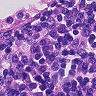
\includegraphics[width=0.3\linewidth]{images/pcam_0_0.png}
		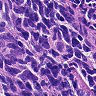
\includegraphics[width=0.3\linewidth]{images/pcam_79_0.png}
		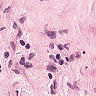
\includegraphics[width=0.3\linewidth]{images/pcam_13_0.png}
		\caption{Negative Examples}
	\end{subfigure}
	\begin{subfigure}{\textwidth}
	\centering
	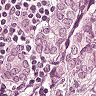
\includegraphics[width=0.3\linewidth]{images/pcam_1_1.png}
	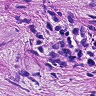
\includegraphics[width=0.3\linewidth]{images/pcam_78_1.png}
	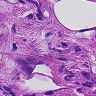
\includegraphics[width=0.3\linewidth]{images/pcam_22_1.png}
	\caption{Positive Examples}
\end{subfigure}
	\caption{Example images from the Patch Cameleyon dataset~\citep{veeling2018rotation,litjens20181399}.}
	\label{fig:pcam_examples}
\end{figure}

\subsection{Experiment Setup}
\label{subsec:unsupervised_experiment}
In order to evaluate the proposed multi-directional contrastive predictive coding approach, an ablation study was conducted using different combinations of the single or multi-directional autoregressive models, and top-down or in-filling style latent masks. To evaluate the learned representations from the CPC models, the trained encoders were used to initialise the encoder weights of 9 CNN classifiers. These CNN classifiers were then trained on a smaller, annotated subset of the training data, which was varied in size from 10 to 100,000 patches in logarithmic scale. This was repeated 3 times, each time with a different subsample of the training data to validate the robustness of the results. The test set was held static across all experiments.

\subsection{Training Parameters}
\label{subsec:unsupervised_training}
In this study, the Contrastive Predictive Coding (CPC) models were trained using a method that involved splitting each input image into overlapping 24x24 patches that were overlapped by 12 pixels. A ResNeXt architecture~\citep{xie2017aggregated} with 101 layers was utilized as the encoder, followed by an additional convolutional layer to produce a 128-dimensional feature vector for each 24x24 patch in the image. The autoregressive model of the CPC was composed of 6 masked convolutional blocks to produce the context vector and predict the masked feature vectors. Additionally, 16 randomly selected images were used as negative samples for the CPC InfoNCE loss function.

The Adam optimisation algorithm was utilised to train the CPC and CNN models, with an initial learning rate of 1e-4. The Adam optimiser~\citep{kingma2014adam} is based on adaptive estimation of first and second-order moments in the parameter gradients to adjust the learning rate during training. The CPC model was trained for 10 epochs with a batch size of 64 and the CNN models were trained for 50 epochs with a batch size of 258. 20\% of the available training data was used as the validation set to prevent overfitting, and early stopping was implemented by saving the model when the loss was lowest on the validation set. 

The CPC models took an average of 33 hours to train using a single Nvidia GeForce RTX 2080 Ti~\footnote{NVIDIA GeForce RTX 2080 Ti: \url{www.nvidia.com/en-gb/geforce/20-series/}} using 16-bit precision. The training loss over the epochs (Figure~\ref{fig:cpc_training}) suggests that the use of a multi-directional autoregressive model was more efficient at reducing the InfoNCE loss than a single-directional top-down autoregressive model. The in-filling style latent mask in combination with the multi-directional autoregressive model stabilized the CPC training process.

\begin{figure}[h]
	\centering
	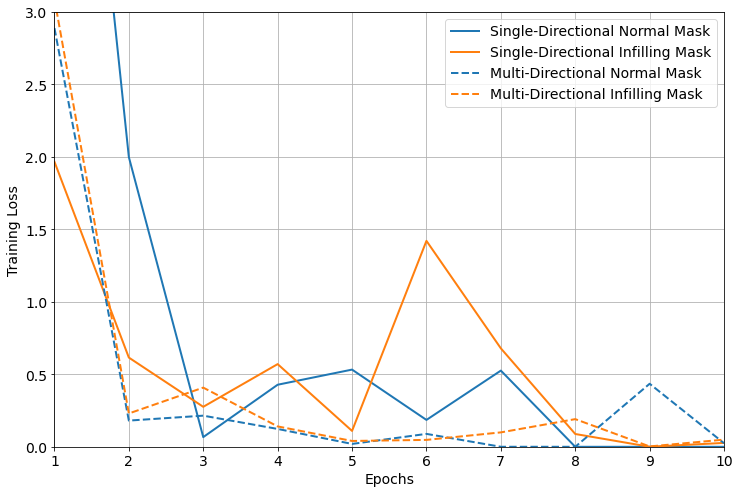
\includegraphics[width=\textwidth]{images/cpc_training.png}
	\caption{Training loss each epoch with the CPC Models.}
	\label{fig:cpc_training}
\end{figure}

\subsection{Results}
\label{subsec:unsupervised_results}
The results of the held-out testing set (32,768 images) for CNN classifiers trained using different CPC encoder's weights and biases for initialization are illustrated in Figure~\ref{fig:cpc_cnn_results} and Table~\ref{tab:cpc_cnn_results}. A baseline with CNN models that have had no pretraining was also included in the study. The findings indicate that the CNNs where small amounts of annotated data were used to train were able to achieve higher accuracies when a multi-directional autoregressive model is employed for initialization. In contrast, standard CPC struggled to learn a representation suitable for initializing a CNN classifier, sometimes resulting in lower accuracies compared to those initialized using random weights. The benefit of using the CPC pretraining decreases as the number of images increases, suggesting that this method of transfer learning is most effective when the number of annotated images is low.

\begin{figure}[h]
	\centering
	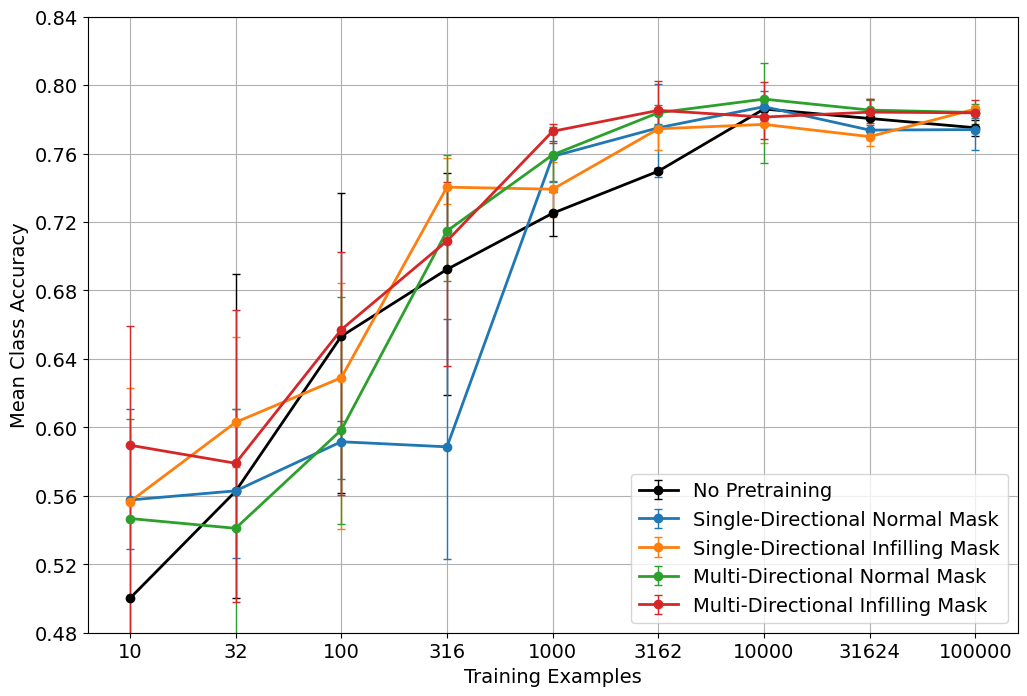
\includegraphics[width=\textwidth]{images/cpc_cnn_results.png}
	\caption{Mean class testing accuracies of the CNN classifiers trained using varying amounts of training examples, with standard errors.}
	\label{fig:cpc_cnn_results}
\end{figure}

\begin{table}[t]
	\centering
	\caption{Mean test accuracies of the CNN classifiers with different pre-training (standard deviation in parentheses).}
	\label{tab:cpc_cnn_results}
	\resizebox{\textwidth}{!}{%
		\begin{tabular}{r|rrrrr}
			\multicolumn{1}{c|}{\begin{tabular}[c]{@{}c@{}}Training\\ Examples\end{tabular}} &
			\multicolumn{1}{c}{\begin{tabular}[c]{@{}c@{}}No \\ Pretraining\end{tabular}} &
			\multicolumn{1}{c}{\begin{tabular}[c]{@{}c@{}}Single\\Directional\\Normal Mask\end{tabular}} &
			\multicolumn{1}{c}{\begin{tabular}[c]{@{}c@{}}Single\\Directional\\Infilling Mask\end{tabular}} &
			\multicolumn{1}{c}{\begin{tabular}[c]{@{}c@{}}Multi\\Directional\\Normal Mask\end{tabular}} &
			\multicolumn{1}{c}{\begin{tabular}[c]{@{}c@{}}Multi\\Directional\\Infilling Mask\end{tabular}} \\ \hline
			10     & 0.500 (0.000) & 0.561 (0.043)          & 0.561 (0.094)          & 0.546 (0.065)          & \textbf{0.582 (0.096)} \\
			32     & 0.563 (0.109) & 0.560 (0.045)          & \textbf{0.604 (0.043)} & 0.538 (0.082)          & 0.577 (0.086)          \\
			100    & 0.641 (0.125) & 0.590 (0.018)          & 0.636 (0.082)          & 0.595 (0.078)          & \textbf{0.655 (0.081)} \\
			316    & 0.694 (0.067) & 0.593 (0.109)          & \textbf{0.741 (0.014)} & 0.715 (0.039)          & 0.708 (0.062)          \\
			1000   & 0.727 (0.013) & 0.758 (0.014)          & 0.740 (0.016)          & 0.760 (0.016)          & \textbf{0.773 (0.006)} \\
			3162   & 0.750 (0.002) & 0.777 (0.028)          & 0.775 (0.012)          & 0.784 (0.006)          & \textbf{0.786 (0.014)} \\
			10000  & 0.786 (0.006) & 0.787 (0.008)          & 0.776 (0.012)          & \textbf{0.792 (0.033)} & 0.781 (0.019)          \\
			31624  & 0.779 (0.012) & 0.774 (0.004)          & 0.770 (0.009)          & \textbf{0.786 (0.005)} & 0.784 (0.009)          \\
			100000 & 0.775 (0.007) & 0.774 (0.011)          & \textbf{0.786 (0.003)} & 0.785 (0.006)          & 0.784 (0.010)
		\end{tabular}%
	}
\end{table}


\section{Conclusion}
\label{sec:conclusion}
The experimental results presented in Section~\ref{subsec:unsupervised_results} demonstrate that the original implementation of Contrastive Predictive Coding (CPC)~\citep{oord2018representation} does not perform well on patch-based digital pathology tasks. The proposed multi-directional modifications to the CPC, however, yielded better results and improved classification accuracies when annotated data were limited. These experiments illustrate that algorithms based on an assumption of image directionality, as is common in standard computer vision datasets such as CIFAR~\citep{krizhevsky2009learning} and ImageNet~\citep{deng2009imagenet}, may not perform well on images without such directionality. The results of this study suggest that the proposed multi-directional CPC method can be applied to other visual tasks where image orientation is unimportant, as is the case in multiple biomedical imaging settings.